\documentclass{article}

\usepackage{arxiv}

\usepackage[utf8]{inputenc} % allow utf-8 input
\usepackage[T1]{fontenc}    % use 8-bit T1 fonts
\usepackage{lmodern}        % https://github.com/rstudio/rticles/issues/343
\usepackage{hyperref}       % hyperlinks
\usepackage{url}            % simple URL typesetting
\usepackage{booktabs}       % professional-quality tables
\usepackage{amsfonts}       % blackboard math symbols
\usepackage{nicefrac}       % compact symbols for 1/2, etc.
\usepackage{microtype}      % microtypography
\usepackage{graphicx}

\title{easystats: A Unified Framework for Statistical Analysis in R}

\author{
    Daniel Lüdecke
   \\
    University Medical Center Hamburg-Eppendorf, Germany \\
   \\
  \texttt{} \\
   \And
    Mattan S. Ben-Shachar
   \\
    Independent Researcher, Ramat Gan, Israel \\
   \\
  \texttt{} \\
   \And
    Indrajeet Patil
   \\
    Carl Zeiss AG, Munich, Germany \\
   \\
  \texttt{} \\
   \And
    Brenton M. Wiernik
   \\
    Independent Researcher, Tampa, FL, USA \\
   \\
  \texttt{} \\
   \And
    Etienne Bacher
   \\
    Luxembourg Institute of Socio-Economic Research (LISER),
Luxembourg \\
   \\
  \texttt{} \\
   \And
    Rémi Thériault
   \\
    Department of Psychology, New York University, New York, NY, USA \\
   \\
  \texttt{} \\
   \And
    Philip D. Waggoner
   \\
    School of Medicine, Stanford University, Stanford, CA, USA \\
   \\
  \texttt{} \\
   \And
    Dominique Makowski
   \\
    School of Psychology, University of Sussex, Brighton, UK \\
   \\
  \texttt{} \\
  }

% Pandoc syntax highlighting
\usepackage{color}
\usepackage{fancyvrb}
\newcommand{\VerbBar}{|}
\newcommand{\VERB}{\Verb[commandchars=\\\{\}]}
\DefineVerbatimEnvironment{Highlighting}{Verbatim}{commandchars=\\\{\}}
% Add ',fontsize=\small' for more characters per line
\usepackage{framed}
\definecolor{shadecolor}{RGB}{248,248,248}
\newenvironment{Shaded}{\begin{snugshade}}{\end{snugshade}}
\newcommand{\AlertTok}[1]{\textcolor[rgb]{0.94,0.16,0.16}{#1}}
\newcommand{\AnnotationTok}[1]{\textcolor[rgb]{0.56,0.35,0.01}{\textbf{\textit{#1}}}}
\newcommand{\AttributeTok}[1]{\textcolor[rgb]{0.13,0.29,0.53}{#1}}
\newcommand{\BaseNTok}[1]{\textcolor[rgb]{0.00,0.00,0.81}{#1}}
\newcommand{\BuiltInTok}[1]{#1}
\newcommand{\CharTok}[1]{\textcolor[rgb]{0.31,0.60,0.02}{#1}}
\newcommand{\CommentTok}[1]{\textcolor[rgb]{0.56,0.35,0.01}{\textit{#1}}}
\newcommand{\CommentVarTok}[1]{\textcolor[rgb]{0.56,0.35,0.01}{\textbf{\textit{#1}}}}
\newcommand{\ConstantTok}[1]{\textcolor[rgb]{0.56,0.35,0.01}{#1}}
\newcommand{\ControlFlowTok}[1]{\textcolor[rgb]{0.13,0.29,0.53}{\textbf{#1}}}
\newcommand{\DataTypeTok}[1]{\textcolor[rgb]{0.13,0.29,0.53}{#1}}
\newcommand{\DecValTok}[1]{\textcolor[rgb]{0.00,0.00,0.81}{#1}}
\newcommand{\DocumentationTok}[1]{\textcolor[rgb]{0.56,0.35,0.01}{\textbf{\textit{#1}}}}
\newcommand{\ErrorTok}[1]{\textcolor[rgb]{0.64,0.00,0.00}{\textbf{#1}}}
\newcommand{\ExtensionTok}[1]{#1}
\newcommand{\FloatTok}[1]{\textcolor[rgb]{0.00,0.00,0.81}{#1}}
\newcommand{\FunctionTok}[1]{\textcolor[rgb]{0.13,0.29,0.53}{\textbf{#1}}}
\newcommand{\ImportTok}[1]{#1}
\newcommand{\InformationTok}[1]{\textcolor[rgb]{0.56,0.35,0.01}{\textbf{\textit{#1}}}}
\newcommand{\KeywordTok}[1]{\textcolor[rgb]{0.13,0.29,0.53}{\textbf{#1}}}
\newcommand{\NormalTok}[1]{#1}
\newcommand{\OperatorTok}[1]{\textcolor[rgb]{0.81,0.36,0.00}{\textbf{#1}}}
\newcommand{\OtherTok}[1]{\textcolor[rgb]{0.56,0.35,0.01}{#1}}
\newcommand{\PreprocessorTok}[1]{\textcolor[rgb]{0.56,0.35,0.01}{\textit{#1}}}
\newcommand{\RegionMarkerTok}[1]{#1}
\newcommand{\SpecialCharTok}[1]{\textcolor[rgb]{0.81,0.36,0.00}{\textbf{#1}}}
\newcommand{\SpecialStringTok}[1]{\textcolor[rgb]{0.31,0.60,0.02}{#1}}
\newcommand{\StringTok}[1]{\textcolor[rgb]{0.31,0.60,0.02}{#1}}
\newcommand{\VariableTok}[1]{\textcolor[rgb]{0.00,0.00,0.00}{#1}}
\newcommand{\VerbatimStringTok}[1]{\textcolor[rgb]{0.31,0.60,0.02}{#1}}
\newcommand{\WarningTok}[1]{\textcolor[rgb]{0.56,0.35,0.01}{\textbf{\textit{#1}}}}

% tightlist command for lists without linebreak
\providecommand{\tightlist}{%
  \setlength{\itemsep}{0pt}\setlength{\parskip}{0pt}}


% Pandoc citation processing
%From Pandoc 3.1.8
% definitions for citeproc citations
\NewDocumentCommand\citeproctext{}{}
\NewDocumentCommand\citeproc{mm}{%
  \begingroup\def\citeproctext{#2}\cite{#1}\endgroup}
\makeatletter
 % allow citations to break across lines
 \let\@cite@ofmt\@firstofone
 % avoid brackets around text for \cite:
 \def\@biblabel#1{}
 \def\@cite#1#2{{#1\if@tempswa , #2\fi}}
\makeatother
\newlength{\cslhangindent}
\setlength{\cslhangindent}{1.5em}
\newlength{\csllabelwidth}
\setlength{\csllabelwidth}{3em}
\newenvironment{CSLReferences}[2] % #1 hanging-indent, #2 entry-spacing
 {\begin{list}{}{%
  \setlength{\itemindent}{0pt}
  \setlength{\leftmargin}{0pt}
  \setlength{\parsep}{0pt}
  % turn on hanging indent if param 1 is 1
  \ifodd #1
   \setlength{\leftmargin}{\cslhangindent}
   \setlength{\itemindent}{-1\cslhangindent}
  \fi
  % set entry spacing
  \setlength{\itemsep}{#2\baselineskip}}}
 {\end{list}}
\usepackage{calc}
\newcommand{\CSLBlock}[1]{#1\hfill\break}
\newcommand{\CSLLeftMargin}[1]{\parbox[t]{\csllabelwidth}{#1}}
\newcommand{\CSLRightInline}[1]{\parbox[t]{\linewidth - \csllabelwidth}{#1}\break}
\newcommand{\CSLIndent}[1]{\hspace{\cslhangindent}#1}

\begin{document}
\maketitle


\begin{abstract}

\end{abstract}

\keywords{
    R; easystats
  }

\section{Summary}\label{summary}

The \textbf{easystats} project is a collection of R packages that
provides a unified and intuitive framework for data wrangling and
statistical analysis. They implement functionalities designed to be
\emph{user-friendly} (e.g., transparent names of functions and
arguments, comprehensive documentation, sensible defaults),
\emph{consistent} (similar syntax and design principles across
packages), and \emph{interoperable} (seamless integration between
packages).

The packages are specialized for different stages of the statistical
workflow, such as data wrangling (\texttt{\{datawizard\}}, Patil et al.,
2022), model assessment (\texttt{\{performance\}}, Lüdecke, Ben-Shachar,
et al., 2021), understanding and describing model parameters
(\texttt{\{parameters\}}, Lüdecke et al., 2020), including Bayesian
models (\texttt{\{bayestestR\}}, Makowski, Ben-Shachar, \& Lüdecke,
2019; Makowski, Ben-Shachar, Chen, et al., 2019), computation of effect
sizes (\texttt{\{effectsize\}}, Ben-Shachar et al., 2020), calculating
and visualizing marginal effects (\texttt{\{modelbased\}}, Makowski et
al., 2025), and generating publication-ready figures (\texttt{\{see\}},
Lüdecke, Patil, et al., 2021) or reports of statistical models
(\texttt{\{report\}}, Makowski et al., 2023).

\section{Statement of Need}\label{statement-of-need}

R is a powerful language for statistical computing, but its capabilities
are scattered across a fragmented landscape of packages. Conducting a
full analysis consisting of data manipulation, modeling, diagnostics,
interpretation, and visualization, often requires juggling multiple
tools with different syntax, design principles, outputs, and classes.
This creates barriers for newcomers and inefficiencies even for
experienced users.

The \textbf{easystats} ecosystem addresses this challenge by enabling a
seamless workflow from data exploration to result communication, while
nudging users toward good, reproducible and transparent statistical
practices with sensible defaults and clear documentation. The packages
in this ecosystem share consistent syntax and integrate seamlessly,
making robust analysis more accessible while reducing cognitive load for
novice and experienced R users alike.

The modular and lightweight nature of the \textbf{easystats} ecosystem
enables developers to use and integrate in other packages only the
necessary components. For example, \texttt{\{insight\}}, a
dependency-free package for retrieving model information, is utilized by
45 other CRAN packages, such as \texttt{\{marginaleffects\}}
(Arel-Bundock et al., 2024) and \texttt{\{gtsummary\}} (Sjoberg et al.,
2021). In contrast, the \texttt{\{easystats\}} meta-package provides
users with a cohesive experience, granting access to the entire
ecosystem and its consistent design principles without needing to know
the specific package of each function.

\section{State of the field}\label{state-of-the-field}

Other R ecosystems or packages often serve different purposes. The
\texttt{\{tidyverse\}} (Wickham et al., 2019), for example, provides
foundational framework for data manipulation and visualisation but does
not focus on the intricacies of statistical model interpretation and
reporting. Specialist packages like \texttt{\{lme4\}} (Bates et al.,
2015) for mixed-effects models or \texttt{\{brms\}} (Bürkner, 2017) for
Bayesian analysis are essential tools, but \textbf{easystats} serves as
a complementary meta-layer that provides a single, easy-to-learn
interface for interacting with the outputs from these and many other
modeling packages. This allows analysts and researchers to focus on
scientific questions rather than the technical idiosyncrasies of
software implementations. \textbf{easystats} meets a critical need when
doing statistics in R by delivering a coherent, intuitive suite of tools
that span the statistical modeling pipeline.

\section{Software design: A Harmonized and Integrated
Workflow}\label{software-design-a-harmonized-and-integrated-workflow}

A key design principle of the \textbf{easystats} ecosystem is the
harmonization and integration of different packages into a simple,
sequential workflow. The typical workflow for a statistical analysis
using \texttt{\{easystats\}} starts with importing data and bringing the
data into shape for the next step---fitting a model---and then
sequentially using different functions to obtain a comprehensive
understanding of the model. This can include checking the model's
parameters, performance metrics, specific effect sizes (e.g.,
Ben-Shachar et al., 2023), and statistical outliers (Thériault et al.,
2024), as well as obtaining publication-ready figures and written
summaries of the results.

\pagebreak

Let's demonstrate this with an example, where the user wants to fit a
mixed effects model:

\begin{Shaded}
\begin{Highlighting}[]
\CommentTok{\# we don\textquotesingle{}t load each package individually,}
\CommentTok{\# but rather the entire ecosystem}
\FunctionTok{library}\NormalTok{(easystats)}
\FunctionTok{data}\NormalTok{(fish, }\AttributeTok{package =} \StringTok{"modelbased"}\NormalTok{)}

\CommentTok{\# rename variable}
\NormalTok{fish }\OtherTok{\textless{}{-}} \FunctionTok{data\_rename}\NormalTok{(fish, }\AttributeTok{select =} \FunctionTok{c}\NormalTok{(}\AttributeTok{treat =} \StringTok{"camper"}\NormalTok{))}

\CommentTok{\# fit mixed model}
\NormalTok{model }\OtherTok{\textless{}{-}}\NormalTok{ glmmTMB}\SpecialCharTok{::}\FunctionTok{glmmTMB}\NormalTok{(}
\NormalTok{  count }\SpecialCharTok{\textasciitilde{}}\NormalTok{ treat }\SpecialCharTok{*}\NormalTok{ persons }\SpecialCharTok{+}\NormalTok{ (}\DecValTok{1} \SpecialCharTok{|}\NormalTok{ ID),}
  \AttributeTok{data =}\NormalTok{ fish,}
  \AttributeTok{family =} \FunctionTok{poisson}\NormalTok{()}
\NormalTok{)}
\end{Highlighting}
\end{Shaded}

The \texttt{model} object can then be passed to functions from different
\textbf{easystats} packages. For instance, the user can get a summary of
the model parameters using the \texttt{\{parameters\}} package:

\begin{Shaded}
\begin{Highlighting}[]
\FunctionTok{model\_parameters}\NormalTok{(model)}
\CommentTok{\#\textgreater{} \# Fixed Effects}
\CommentTok{\#\textgreater{} }
\CommentTok{\#\textgreater{} Parameter           | Log{-}Mean |   SE |         95\% CI |     z |      p}
\CommentTok{\#\textgreater{} {-}{-}{-}{-}{-}{-}{-}{-}{-}{-}{-}{-}{-}{-}{-}{-}{-}{-}{-}{-}{-}{-}{-}{-}{-}{-}{-}{-}{-}{-}{-}{-}{-}{-}{-}{-}{-}{-}{-}{-}{-}{-}{-}{-}{-}{-}{-}{-}{-}{-}{-}{-}{-}{-}{-}{-}{-}{-}{-}{-}{-}{-}{-}{-}{-}{-}{-}{-}{-}{-}{-}}
\CommentTok{\#\textgreater{} (Intercept)         |    {-}0.74 | 0.32 | [{-}1.36, {-}0.12] | {-}2.33 | 0.020 }
\CommentTok{\#\textgreater{} treat [1]           |    {-}0.83 | 0.29 | [{-}1.41, {-}0.25] | {-}2.81 | 0.005 }
\CommentTok{\#\textgreater{} persons             |     0.39 | 0.07 | [ 0.24,  0.53] |  5.25 | \textless{} .001}
\CommentTok{\#\textgreater{} treat [1] × persons |     0.60 | 0.09 | [ 0.42,  0.77] |  6.78 | \textless{} .001}
\CommentTok{\#\textgreater{} }
\CommentTok{\#\textgreater{} \# Random Effects}
\CommentTok{\#\textgreater{} }
\CommentTok{\#\textgreater{} Parameter          | Coefficient |       95\% CI}
\CommentTok{\#\textgreater{} {-}{-}{-}{-}{-}{-}{-}{-}{-}{-}{-}{-}{-}{-}{-}{-}{-}{-}{-}{-}{-}{-}{-}{-}{-}{-}{-}{-}{-}{-}{-}{-}{-}{-}{-}{-}{-}{-}{-}{-}{-}{-}{-}{-}{-}{-}{-}}
\CommentTok{\#\textgreater{} SD (Intercept: ID) |        0.42 | [0.20, 0.86]}
\end{Highlighting}
\end{Shaded}

Then, the performance of the model can be assessed with the
\texttt{\{performance\}} package:

\begin{Shaded}
\begin{Highlighting}[]
\FunctionTok{model\_performance}\NormalTok{(}
\NormalTok{  model,}
  \AttributeTok{metrics =} \FunctionTok{c}\NormalTok{(}\StringTok{"AIC"}\NormalTok{, }\StringTok{"BIC"}\NormalTok{, }\StringTok{"R2"}\NormalTok{)}
\NormalTok{)}
\CommentTok{\#\textgreater{} \# Indices of model performance}
\CommentTok{\#\textgreater{} }
\CommentTok{\#\textgreater{} AIC    |    BIC | R2 (cond.) | R2 (marg.)}
\CommentTok{\#\textgreater{} {-}{-}{-}{-}{-}{-}{-}{-}{-}{-}{-}{-}{-}{-}{-}{-}{-}{-}{-}{-}{-}{-}{-}{-}{-}{-}{-}{-}{-}{-}{-}{-}{-}{-}{-}{-}{-}{-}{-}{-}{-}}
\CommentTok{\#\textgreater{} 2375.5 | 2393.1 |      0.796 |      0.661}
\end{Highlighting}
\end{Shaded}

The results can be visualized using the \texttt{\{see\}} package by, for
example, plotting the model's predictions from \texttt{\{modelbased\}}
(Figure 1):

\begin{Shaded}
\begin{Highlighting}[]
\NormalTok{predictions }\OtherTok{\textless{}{-}} \FunctionTok{estimate\_means}\NormalTok{(model, }\FunctionTok{c}\NormalTok{(}\StringTok{"persons"}\NormalTok{, }\StringTok{"treat"}\NormalTok{))}
\FunctionTok{plot}\NormalTok{(predictions) }\SpecialCharTok{+}
  \FunctionTok{theme\_modern}\NormalTok{(}\AttributeTok{show.ticks =} \ConstantTok{TRUE}\NormalTok{) }\SpecialCharTok{+} \CommentTok{\# add nice theme}
  \FunctionTok{scale\_color\_material}\NormalTok{() }\CommentTok{\# add some nice colors}
\end{Highlighting}
\end{Shaded}

\begin{figure}
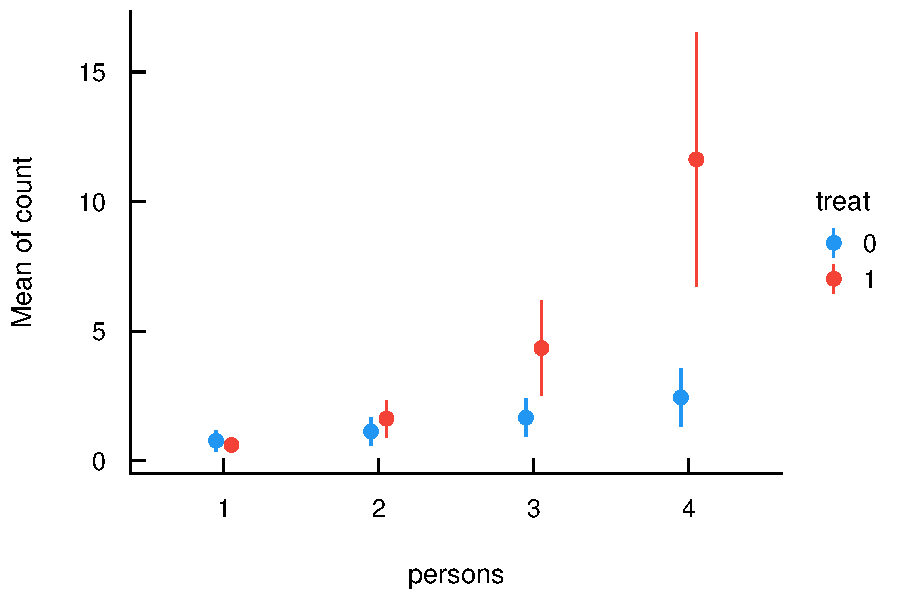
\includegraphics[width=1\linewidth]{paper_files/figure-latex/fig1-1} \caption{Predicted probability of alertness by treatment group.}\label{fig:fig1}
\end{figure}

\pagebreak

Finally, a full report of the analysis can be generated with the
\texttt{\{report\}} package:

\begin{Shaded}
\begin{Highlighting}[]
\FunctionTok{report}\NormalTok{(model)}
\CommentTok{\#\textgreater{} We fitted a poisson mixed model (estimated using ML and nlminb}
\CommentTok{\#\textgreater{} optimizer) to predict count with treat and persons (formula: count \textasciitilde{}}
\CommentTok{\#\textgreater{} treat * persons). The model included ID as random effect (formula:}
\CommentTok{\#\textgreater{} \textasciitilde{}1 | ID). The model\textquotesingle{}s total explanatory power is substantial}
\CommentTok{\#\textgreater{} (conditional R2 = 0.80) and the part related to the fixed effects}
\CommentTok{\#\textgreater{} alone (marginal R2) is of 0.66. The model\textquotesingle{}s intercept, corresponding}
\CommentTok{\#\textgreater{} to treat = 0 and persons = 0, is at {-}0.74 (95\% CI [{-}1.36, {-}0.12], p}
\CommentTok{\#\textgreater{} = 0.020). Within this model:}
\CommentTok{\#\textgreater{} }
\CommentTok{\#\textgreater{}   {-} The effect of treat [1] is statistically significant and negative}
\CommentTok{\#\textgreater{} (beta = {-}0.83, 95\% CI [{-}1.41, {-}0.25], p = 0.005)}
\CommentTok{\#\textgreater{}   {-} The effect of persons is statistically significant and positive}
\CommentTok{\#\textgreater{} (beta = 0.39, 95\% CI [0.24, 0.53], p \textless{} .001)}
\CommentTok{\#\textgreater{}   {-} The effect of treat [1] × persons is statistically significant and}
\CommentTok{\#\textgreater{} positive (beta = 0.60, 95\% CI [0.42, 0.77], p \textless{} .001)}
\CommentTok{\#\textgreater{} }
\CommentTok{\#\textgreater{} Standardized parameters were obtained by fitting the model on a}
\CommentTok{\#\textgreater{} standardized version of the dataset. 95\% Confidence Intervals (CIs)}
\CommentTok{\#\textgreater{} and p{-}values were computed using a Wald z{-}distribution}
\CommentTok{\#\textgreater{} approximation.}
\end{Highlighting}
\end{Shaded}

The \texttt{model\_dashboard()} function generates an interactive model
summary, integrating several \textbf{easystats} steps into a single
command. Since this paper is a static document, Figure 2 provides a
static screenshot of the interactive report.

\begin{figure}
\centering
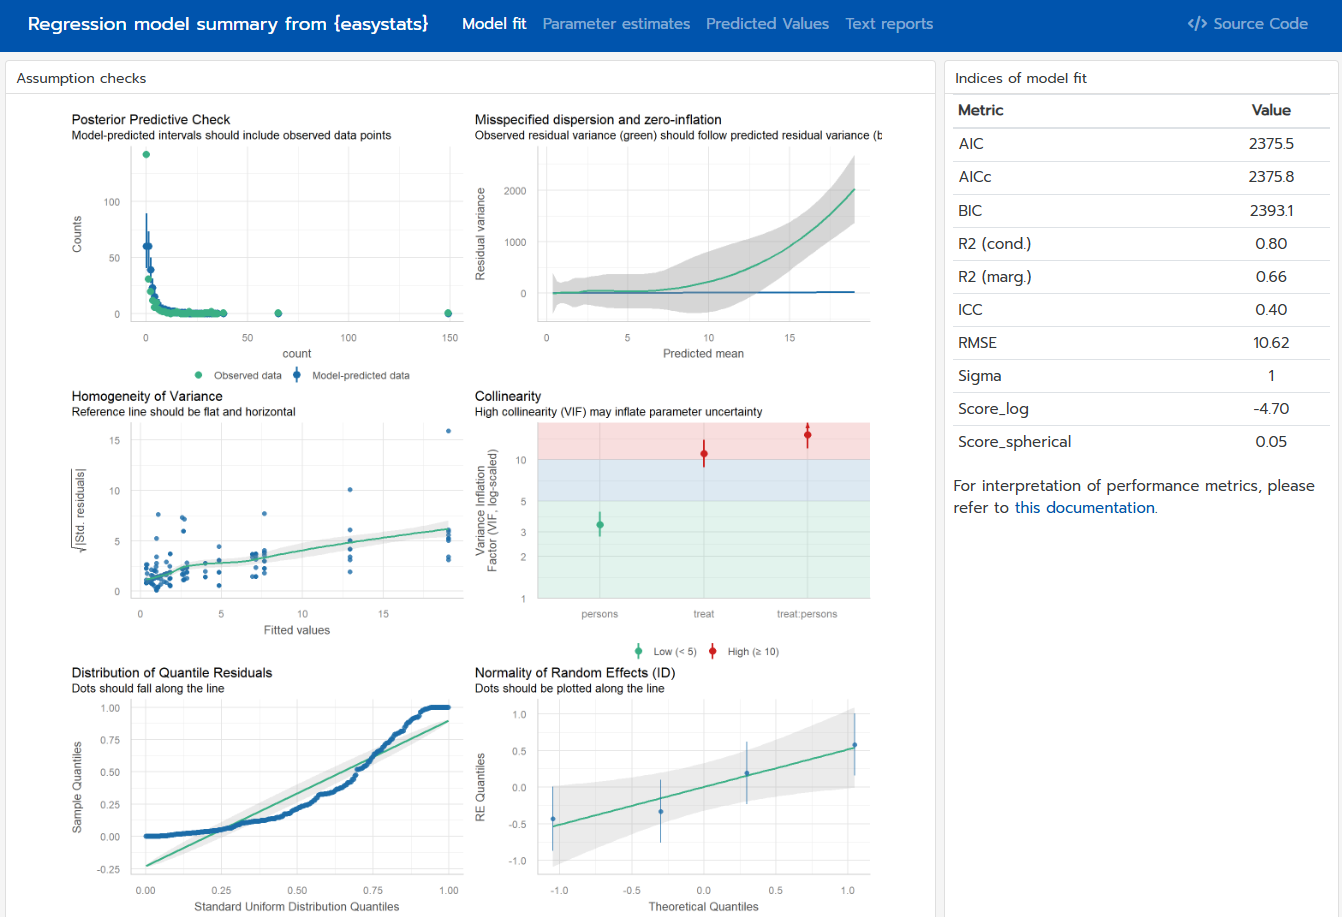
\includegraphics[width=1\linewidth,height=\textheight,keepaspectratio,alt={Screenshot of the ``Model fit'' tab from the interactive dashboard}]{paper_files/dashboard.png}
\caption{Screenshot of the ``Model fit'' tab from the interactive
dashboard}
\end{figure}

This seamless integration between \textbf{easystats} packages allows
users to move from model fitting and interpretation to visualization and
reporting in a fluid and intuitive way, without having to learn
different syntaxes, data structures, or idiosyncratic software design
choices.

To get the newest features from the rapidly developing
\textbf{easystats} ecosystem, users can run
\texttt{easystats::install\_latest()}. It conveniently installs the
latest development version of every package in the project.

\section{Research impact statement}\label{research-impact-statement}

The \textbf{easystats} ecosystem has a substantial realized impact
across the scientific community, as shown by the high citation counts of
its related publications only from the Journal of Open Source Software.
For example, the \texttt{\{performance\}} and \texttt{\{bayestestR\}}
packages alone have over 6,000 and 1,600 citations, respectively
(statistic from February 2026). Because a typical analysis leverages
multiple \textbf{easystats} packages sequentially throughout the
statistical workflow, this meta-package paper provides researchers with
a single, unified citation to streamline referencing and to avoid the
need for excessive citations.

\section{Licensing and Availability}\label{licensing-and-availability}

The release version of \texttt{\{easystats\}} is available for download
from \href{https://doi.org/10.32614/CRAN.package.easystats}{CRAN},
whereas development versions are available from the
\href{https://easystats.r-universe.dev/easystats}{R-universe} and
\href{https://github.com/easystats/easystats/}{GitHub}. The package is
licensed under the MIT-License, with all source code stored at GitHub
(\url{https://github.com/easystats/easystats}), with a corresponding
issue tracker for bug reporting and feature enhancements. In the spirit
of honest and open science, we encourage requests, tips for fixes,
feature updates, as well as general questions and concerns via direct
interaction with contributors and developers.

\section{AI usage disclosure}\label{ai-usage-disclosure}

No generative AI was used in software creation, writing the
documentation or the paper.

\section{Acknowledgments}\label{acknowledgments}

\texttt{\{easystats\}} is part of the collaborative
\href{https://easystats.github.io/easystats/}{\textbf{easystats}
ecosystem}. Thus, we thank all
\href{https://github.com/orgs/easystats/people}{members of easystats},
contributors, and users alike.

\section*{References}\label{references}
\addcontentsline{toc}{section}{References}

\protect\phantomsection\label{refs}
\begin{CSLReferences}{1}{0}
\bibitem[\citeproctext]{ref-arel-bundock_how_2024}
Arel-Bundock, V., Greifer, N., \& Heiss, A. (2024). How to interpret
statistical models using marginaleffects for {R} and {Python}.
\emph{Journal of Statistical Software}, \emph{111}(9).
\url{https://doi.org/10.18637/jss.v111.i09}

\bibitem[\citeproctext]{ref-bates_fitting_2015}
Bates, D., Mächler, M., Bolker, B., \& Walker, S. (2015). Fitting linear
mixed-effects models using lme4. \emph{Journal of Statistical Software},
\emph{67}(1), 1--48. \url{https://doi.org/10.18637/jss.v067.i01}

\bibitem[\citeproctext]{ref-Ben-Shachar2020}
Ben-Shachar, M. S., Lüdecke, D., \& Makowski, D. (2020). {effectsize}:
Estimation of effect size indices and standardized parameters.
\emph{Journal of Open Source Software}, \emph{5}(56), 2815.
\url{https://doi.org/10.21105/joss.02815}

\bibitem[\citeproctext]{ref-ben2023phi}
Ben-Shachar, M. S., Patil, I., Thériault, R., Wiernik, B. M., \&
Lüdecke, D. (2023). Phi, fei, fo, fum: Effect sizes for categorical data
that use the chi-squared statistic. \emph{Mathematics}, \emph{11}(9),
1982. \url{https://doi.org/10.3390/math11091982}

\bibitem[\citeproctext]{ref-burkner2017brms}
Bürkner, P.-C. (2017). Brms: An r package for bayesian multilevel models
using stan. \emph{Journal of Statistical Software}, \emph{80}, 1--28.

\bibitem[\citeproctext]{ref-Luxfcdecke2020parameters}
Lüdecke, D., Ben-Shachar, M. S., Patil, I., \& Makowski, D. (2020).
{parameters}: Extracting, computing and exploring the parameters of
statistical models using {R}. \emph{Journal of Open Source Software},
\emph{5}(53), 2445. \url{https://doi.org/10.21105/joss.02445}

\bibitem[\citeproctext]{ref-Luxfcdecke2020performance}
Lüdecke, D., Ben-Shachar, M. S., Patil, I., Waggoner, P., \& Makowski,
D. (2021). {performance}: An {R} package for assessment, comparison and
testing of statistical models. \emph{Journal of Open Source Software},
\emph{6}(60), 3139. \url{https://doi.org/10.21105/joss.03139}

\bibitem[\citeproctext]{ref-ludecke_see_2021}
Lüdecke, D., Patil, I., Ben-Shachar, M., Wiernik, B., Waggoner, P., \&
Makowski, D. (2021). {see}: An {R} package for visualizing statistical
models. \emph{Journal of Open Source Software}, \emph{6}(64), 3393.
\url{https://doi.org/10.21105/joss.03393}

\bibitem[\citeproctext]{ref-makowski2019indices}
Makowski, D., Ben-Shachar, M. S., Chen, S. A., \& Lüdecke, D. (2019).
Indices of effect existence and significance in the {Bayesian}
framework. \emph{Frontiers in Psychology}, \emph{10}, 2767.
\url{https://doi.org/10.3389/fpsyg.2019.02767}

\bibitem[\citeproctext]{ref-Makowski2019}
Makowski, D., Ben-Shachar, M. S., \& Lüdecke, D. (2019). {bayestestR}:
Describing effects and their uncertainty, existence and significance
within the {Bayesian} framework. \emph{Journal of Open Source Software},
\emph{4}(40), 1541. \url{https://doi.org/10.21105/joss.01541}

\bibitem[\citeproctext]{ref-Makowski2025modelbased}
Makowski, D., Ben-Shachar, M. S., Wiernik, B. M., Patil, I., Thériault,
R., \& Lüdecke, D. (2025). {modelbased}: An {R} package to make the most
out of your statistical models through marginal means, marginal effects,
and model predictions. \emph{Journal of Open Source Software},
\emph{10}(109), 7969. \url{https://doi.org/10.21105/joss.07969}

\bibitem[\citeproctext]{ref-report_remi_2023}
Makowski, D., Lüdecke, D., Patil, I., Thériault, R., Ben-Shachar, M. S.,
\& Wiernik, B. M. (2023). {report}: Automated results reporting as a
practical tool to improve reproducibility and methodological best
practices adoption. \emph{CRAN}.
\url{https://doi.org/10.32614/CRAN.package.report}

\bibitem[\citeproctext]{ref-patil_datawizard_2022}
Patil, I., Makowski, D., Ben-Shachar, M. S., Wiernik, B. M., Bacher, E.,
\& Lüdecke, D. (2022). {datawizard}: An {R} package for easy data
preparation and statistical transformations. \emph{Journal of Open
Source Software}, \emph{7}(78), 4684.
\url{https://doi.org/10.21105/joss.04684}

\bibitem[\citeproctext]{ref-gtsummary2021}
Sjoberg, D. D., Whiting, K., Curry, M., Lavery, J. A., \& Larmarange, J.
(2021). {Reproducible Summary Tables with the gtsummary Package}.
\emph{{The R Journal}}, \emph{13}(1), 570--580.
\url{https://doi.org/10.32614/RJ-2021-053}

\bibitem[\citeproctext]{ref-theriault2024check}
Thériault, R., Ben-Shachar, M. S., Patil, I., Lüdecke, D., Wiernik, B.
M., \& Makowski, D. (2024). Check your outliers! An introduction to
identifying statistical outliers in {R} with easystats. \emph{Behavior
Research Methods}, \emph{56}(4), 4162--4172.
\url{https://doi.org/10.3758/s13428-024-02356-w}

\bibitem[\citeproctext]{ref-Wickham2019}
Wickham, H., Averick, M., Bryan, J., Chang, W., McGowan, L. D.,
François, R., Grolemund, G., Hayes, A., Henry, L., Hester, J., Kuhn, M.,
Pedersen, T. L., Miller, E., Bache, S. M., Müller, K., Ooms, J.,
Robinson, D., Seidel, D. P., Spinu, V., \ldots{} Yutani, H. (2019).
Welcome to the {tidyverse}. \emph{Journal of Open Source Software},
\emph{4}(43), 1686. \url{https://doi.org/10.21105/joss.01686}

\end{CSLReferences}

\bibliographystyle{unsrt}
\bibliography{paper.bib}


\end{document}
